\cotefile{79}
\scanpage{1}
% letterhead
\figure{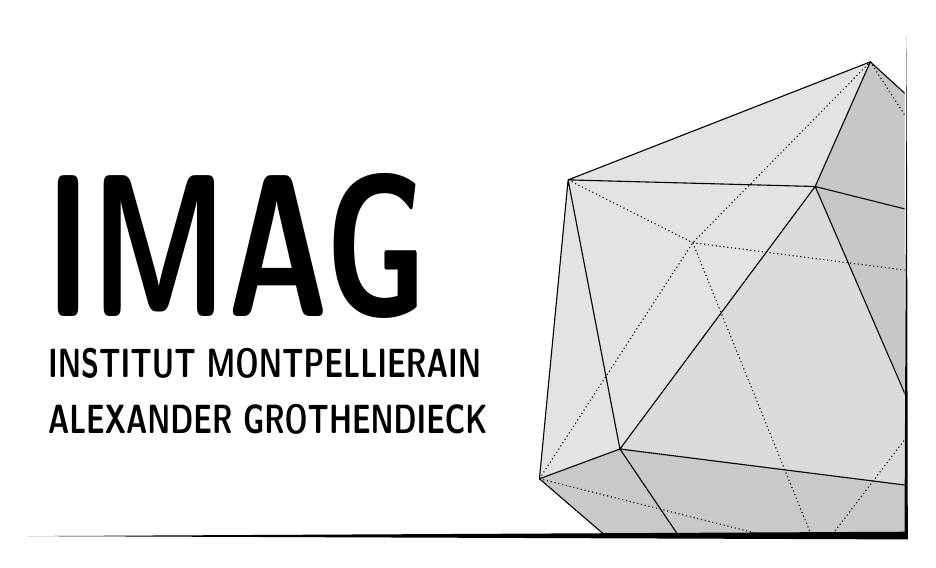
\begin{tikzpicture}[x=.014cm,y=-.014cm,line join=round]
  \node[anchor=west,inner sep=0] at (22,198) {\resizebox{4.84cm}{1.79cm}{\sffamily\bfseries IMAG}};
  \node[anchor=west,inner sep=0] at (24,304) {\resizebox{5.50cm}{.36cm}{\sffamily\bfseries INSTITUT MONTPELLIERAIN}};
  \node[anchor=west,inner sep=0] at (24,355) {\resizebox{5.58cm}{.36cm}{\sffamily\bfseries ALEXANDER GROTHENDIECK}};
  \begin{scope}
  \clip (468,0) rectangle (801,459);
  \fill[black!11] (496,138)--(770,31)--(804,62)--(804,459)--(528,459)--(470,409)--cycle;
  \fill[black!22] (720,144)--(770,31)--(803,62)--(803,333)--cycle;
  \fill[black!14] (543,382)--(720,144)--(803,334)--(803,415)--cycle;
  \fill[black!21] (470,409)--(543,382)--(803,415)--(803,459)--(528,459)--cycle;
  \draw (496,138)--(770,31)--(804,62) (770,31)--(720,144)--(496,138)--(470,409)--(543,382)--(496,138)
        (470,409)--(528,459) (543,382)--(595,459) (543,382)--(804,415)
        (543,382)--(720,144)--(804,165) (720,144)--(804,338);
  \draw[densely dotted] (496,138)--(609,195)--(803,220) (470,409)--(609,195)--(770,31)--(803,82)
        (609,195)--(716,459) (470,409)--(669,459) (736,459)--(803,371);
  \end{scope}
  \fill (6,461)--(801,457)--(803,8)--(804,464)--cycle;
\end{tikzpicture}}
\scanpage{2}
$\deleted{2}2$-polyèdres réguliers triangulés, et modules libres de rang $2$ sur les anneaux $\Lambda=\mathbb{Z}/n\mathbb{Z}$. et $\Lambda=\mathbb{Z}$.
% archive sheet number: 1
\scanpage{3}
I\quad Construction d'un $2$-polyèdre triangulé régulier orienté \ldots\hfill p.~\uline{1}

$\overline{\underline{\mathrm{II}}}$\quad Relation avec l'isom $\mathrm{Gl}(2,\mathbb{Z})\simeq\mathbb{G}_{\infty,3}$\hfill p.~$12'$

$\overline{\underline{\mathrm{III}}}$\quad Cas d'une structure $\frac12$ symplectique variable, sur $M$ : \unsure{recherche|recherches} des structures sur $P^{\deleted{\unsure{\infty|\sim}}}_{\underline M}=(S_M,F_M=\coprod_{i\in\pi}F_{M,i})$.\hfill p.~18

$\overline{\underline{\mathrm{IV}}}$\quad Récapitulation (1)\hfill p.~30

$\overline{\underline{\mathrm{V}}}$\quad Re-récapitulation, avec programme de travail\hfill p.~35

$\overline{\underline{\mathrm{VI}}}$\quad Calcul du commutant de $\mathrm{Sl}_{\Lambda}(\unsure{M|\underline M})$ dans $M^*/\pm1$, et applications\hfill p.~46

$\overline{\underline{\mathrm{VII}}}$\quad Axiomatique des structures triangulaires congruentielles (1)\hfill p.~$51'$

$\overline{\underline{\mathrm{VIII}}}$\quad Axiomatique : reformulation\hfill p.~65

$\overline{\underline{\mathrm{IX}}}$\quad Point de vue graphes à \deleted{\unsure{opérateurs|opérations}, \unsure{de graphes|de pointements}} \inserted{homothéties et multigraphes} à \deleted{\unsure{opérateurs|opérations}} \inserted{homothéties}. \inserted{``Mise en \unsure{équations|graphes}'' \unsure{gruppenthéorétique|groupe-théorétique}\ldots}\hfill p.~81.

$\overline{\underline{\mathrm{X}}}$\quad ``Antipodismes'' en général -- dualité (pour les \deleted{\unsure{ou}} graphes) -- \uline{prégraphes à homothéties}.\hfill p.~92

1. Antipodismes généralisés\hfill \deleted{p.~\unsure{111}} \deleted{\illegible{1}} 92

2. Où les étoiles prennent le pas -- structures de contour \unsure{invariante|invariantes}\dotfill 98 \deleted{\unsure{102}}

3. Présentation symétrique $S,S^\vee$ sur une $\mathbb{Z}/n\mathbb{Z}$-droite affine\dotfill 102

\deleted{4. Retour sur condition d'isomorphisme\hfill \unsure{113}}

$\overline{\underline{\mathrm{XI}}}$\quad \uline{Récapitulation} des notions obtenues\hfill 114

1. Graphes, prégraphes, \unsure{jougs|je-ges|jeux|pages}, multigraphes, \unsure{multizygons|multizygues|multipages} --\hfill 114\qquad --

2. Condition d'isomorphie pour un multigraphe\hfill $120'$

3. Condition d'homogénéité : Traductions \unsure{gruppenthéorétiques|groupe-théorétiques}\hfill \unsure{122|123}

4. Cas des graphes \unsure{triangulaires|triangulants|triangulatoires}.\hfill 13\deleted{\unsure{7}}8

\margin{p.~79/90/95\unsure{$'$|$1$}}
% archive sheet number: 2
\scanpage{4}\mspage{1}
% slanted
\margin{I Construction d'un $2$-polyèdre triangulé orienté régulier, associé à un $\Lambda$-module libre de rang $2$, pour $\Lambda\simeq\mathbb{Z}$ ou $\mathbb{Z}/n\mathbb{Z}$\ldots}

Soit $M$ un module libre de rang $2$ sur un anneau $\Lambda$. \deleted{\unsure{Introduisons|Considérons}} Soit $\{x,y,z\}\in M^3$, tel que
\[
\deleted{\unsure{B}}\quad\deleted{B(M)=\{x,\unsure{y}}
\]
\[
x+y+z=0\tag*{(1)}
\]
alors
\[
\{x,y\}\in\deleted{\unsure{\mathrm{Rep}}}\mathrm{Base}_{\Lambda}(M)\iff\{y,z\}\in\deleted{\unsure{\mathrm{Rep}}}\mathrm{Base}_{\Lambda}(M)\iff\{z,x\}\in\unsure{\mathrm{Bas}|\mathrm{Base}}_{\Lambda}(M)\tag*{(2)}
\]
On désigne par
\[
B(M)\subset M^3\tag*{(3)}
\]
l'ens. des triplets $(x,y,z)$ satisfaisant (1) \deleted{\unsure{et}} \deleted{\unsure{qui}} et les conditions équivalentes de (2).

\deleted{Sur} \inserted{La partie} $B(M)$\deleted{, le \unsure{gr.}} de $M^3$ est stable pour l'action de $\mathfrak{S}_3$ opérant sur $M^3$, et $\mathfrak{S}_3$ opère librement sur $B(M)$. Considérons le quotient
\[
\deleted{\unsure{B(M)}}\quad\widetilde F(M)\overset{\text{déf}}{=}B(M)/\mathfrak{S}_3\simeq
\left\{A\subset\unsure{\mathfrak P|\mathscr P}_3(M)\ \middle|\ 
\begin{gathered}\textstyle\sum_{x\in A}x=0,\\ \forall x\in A,\\ A\setminus\{x\}\in\mathrm{Base}\unsure{(M)}\end{gathered}\right\}\tag*{(4)}
\]
\deleted{\unsure{Soit|Notons}} On peut aussi interpréter $B(M)$ comme can. isom. à l'ens. des \uline{repères} de $M$ i.e. des bases ordonnées $(x,y)$, par
\[
\begin{aligned}
B(M)&\xrightarrow{\sim}\mathrm{Rep}(M)\overset{\text{(déf)}}{=}\mathrm{Isom}_{\Lambda}(\Lambda^2,M)\\
(x,y,z)&\longmapsto (x,y)
\end{aligned}\tag*{(5)}
\]
l'action de $\mathfrak{S}_3$ sur $B(M)$ provient alors d'une action de $\mathfrak{S}_3$ sur $\mathrm{Rep}(M)$, déduite
% archive sheet number: 3
\scanpage{5}
d'une action de $\mathfrak{S}_3$ sur \inserted{le $\Lambda$-module} $\Lambda^2$ qu'on peut expliciter ainsi. On considère l'action de $\mathfrak{S}_3$ sur
\[
\Lambda^3/\underbrace{\Lambda}_{\text{diagonale}}=V'_{\{1,2,3\}}(\Lambda)={}_{2}V'_{\Lambda}\tag*{(6)}
\]
de sorte que l'on a un isom canonique de $\mathfrak{S}_3$-ensembles
\[
\overset{\unsure{\sim|\deleted{\sim}|-}}{B}(M)\simeq\mathrm{Isom}_{\Lambda}(V'_{\Lambda},M)\tag*{(7)}
\]
D'ailleurs \deleted{\unsure{l'is|l'i}} l'application (5) est composée de (7) et de la bijection
\[
\mathrm{Isom}_{\Lambda}(V'_{\Lambda},M)\xrightarrow{\sim}\mathrm{Isom}_{\Lambda}(\Lambda^2,M)
\]
déduit de l'isomorphisme canonique
\[
\left\{\begin{aligned}
\Lambda^2&\xrightarrow{\sim}\Lambda^3/\Lambda\\
(x,y)&\longmapsto(x,y,0)\bmod\Lambda
\end{aligned}\right. \ .\tag*{(8)}
\]
Revenons à un $(x,y,z)\in B(M)$, notons qu'on \unsure{aura|a} alors
\[
x\wedge y=y\wedge z=z\wedge x\ \in
\underbrace{\det(M)^*}_{\substack{\text{ens des}\\\text{bases du }\Lambda\text{-module}\\\text{inversible }\det M=\Lambda^2 M}}\tag*{(9)}
\]
De façon intrinsèque, si $A\in\widetilde F(M)$, \deleted{choisissant un ordre total $(x,y,z)$} \inserted{\unsure{l'écrivant|écrivant} $A=\{x,y,z\}$},
% archive sheet number: 4
\scanpage{6}\mspage{2}
l'élément $x\wedge y$ de $(\det M)^*$ ne dépend que de la permutation circulaire $\omega\in\underline{\omega}_A$ définie par l'ordre total choisi sur $A$, on trouve donc une application canonique
\[
\underline{\omega}_A\xrightarrow{\alpha_A}(\det M)^*\tag*{(10)}
\]
satisfaisant
\[
\alpha_A(\omega^{-1})=-\alpha_A(\omega)\tag*{(11)}
\]
de sorte que $\alpha_A$ peut aussi s'interpréter comme un élément
\[
\alpha_A\in\left(\det_{\Lambda}(M)\wedge_{\mu_2}\underline{\omega}_A\right)^*\simeq
\det_{\Lambda}(M)^*\wedge_{\mu_2}\underline{\omega}_A.\tag*{(12)}
\]
\deleted{On} Si $M$ est ``jaugé'' i.e. muni d'une \uline{base} de $\det M$, soit $e_M$, on pose
\[
\left\{\begin{aligned}
S\widetilde F(M)&=\left\{A\in\widetilde F(M)\mid\alpha_A\in
\underbrace{\{\pm e_M\}\wedge_{\mu_2}\underline{\omega}_A}_{\simeq\,\underline{\omega}_A}\right\}\\
\deleted{S\widetilde F^+(M)}&\deleted{=\{A\in\widetilde F(M)\mid\alpha_A\unsure{\in}\ \in}
\end{aligned}\right.\tag*{(13)}
\]
i.e. $S\widetilde F(M)$ est formé des $A\in\widetilde F(M)$ tels que l'image de $\underline{\omega}_A$ par (\deleted{\unsure{4|1}}10) soit $\{\pm e_M\}$. Si $2\ne0$ dans $\Lambda$, i.e si $\Lambda$ n'est pas une $\mathbb F_2$-algèbre, alors \deleted{(10) est injectif, \unsure{et|donc|dès}}
\[
\alpha_A:\ \underline{\omega}_A\simeq\{\pm e_M\}
\]
est une bijection, ce qui implique que
% archive sheet number: 5
\scanpage{7}
$\underline{\omega}_A$ est muni d'un élément canonique, que je note $\omega_A$, caractérisé par
\[
\left\{\begin{aligned}
&\omega_A\in\underline{\omega}_A,\\
&\alpha_A(\omega_A)=e_M\qquad\text{ou encore}\qquad\alpha_A=e_M\wedge\omega_A
\end{aligned}\right.\tag*{(14)}
\]
Considérons aussi
\[
\begin{aligned}
\widetilde S_M=M^*&\overset{\mathrm{def}}{=}\left\{x\in M\ \middle|\ \begin{gathered}
x(s)\ne0\text{ dans }M(s)\\ \text{pour tout }s\in\mathrm{Spec}\,\Lambda\end{gathered}\right\}\\
&=\left\{x\in M\mid M/\Lambda x\text{ est un }\Lambda\text{-module inversible}\right\}
\end{aligned}\tag*{(15)}
\]
On a \deleted{une application} \inserted{donc l'inclusion}
\[
\widetilde F_M\subset\unsure{\mathfrak P|\mathscr P}_3(\widetilde S_M=M^*)\tag*{(\deleted{\unsure{6|(}}16)}
\]
et on a en fait
\[
\left\{\begin{aligned}
&\text{Si }\mathrm{Pic}(\Lambda)=0\qquad\text{p.ex. si }\Lambda\ \tfrac12\text{ local}\\
&\text{alors}\quad\widetilde S_M=M^*=\{x\in M\mid\exists\, A\in\widetilde F_M,\ x\in A\}\\
&\text{i.e.}\quad\widetilde S_M=\bigcup_{A\in\widetilde F_M} A
\end{aligned}\right.\tag*{(17)}
\]
Ainsi, $\widetilde S_M$ apparaît comme la réunion d'une ensemble \inserted{$\widetilde F_M$} de parties à trois éléments, et on voit tout de suite que si $\{x,y\}\in\mathfrak P_2(\widetilde S_M)$, alors il existe au plus \uline{un} $A\in\widetilde F_M$ le contenant.
% archive sheet number: 6
\scanpage{8}\mspage{3}
Notons que $\mathrm{Gl}_{\Lambda}(M)$ opère sur $\widetilde S_M$, en stabilisant $\widetilde F_M$, et $\mathrm{Sl}_{\Lambda}(M)$ opère en stabilisant de plus le système des $\alpha_A\in\underline{\omega}_A$, $A\in\widetilde F_M$.

\deleted{Considérons maintenant les ens.}

Considérons en particulier l'action de \inserted{l'involution} $-\mathrm{id}_M$ sur $\widetilde S_M$, qui (si $2\,1_{\Lambda}\ne0$) opère sans points fixes sur $\widetilde S_M$. On pose
\[
\left\{\begin{aligned}
S_M&=\widetilde S_M/\{\pm\mathrm{id}_M\}\\
F_M&=\widetilde F_M/\{\pm\mathrm{id}_M\}.
\end{aligned}\right.\tag*{(18)}
\]
Notons que si $\{x,y,z\}\in\widetilde F_M$, alors $y\ne\pm x$, $z\ne\pm y$, $x\ne\pm z$, i.e. $\{\dot x,\dot y,\dot z\}\in\unsure{\mathfrak P|\mathscr P}_3(S_M)$. On trouve ainsi une application
\[
F_M\longrightarrow\mathfrak P_3(S_M)
\]
je dis que celle-ci est injective, en d'autres termes, \inserted{si $\deleted{\unsure{(}}\{x,y,z\}\inS_F$ et} si $\varepsilon,\varepsilon',\varepsilon''$ \inserted{$\in\{\pm1\}_{\Lambda}$} \deleted{sont des signes} sont des signes qui ne sont pas tous égaux, alors on ne peut avoir
\[
\deleted{\unsure{\{}}\{\varepsilon x,\varepsilon'\deleted{\unsure{z}}y,\varepsilon''z\}\in\overset{\sim}{\deleted{\unsure{S}}F}_M.
\]
OPS que $\varepsilon,\varepsilon'=+1$, $\varepsilon''=-1$, et il faut montrer
% archive sheet number: 7
\scanpage{9}
qu'on ne peut avoir simultanément
\[
\{x,y,z\},\ \{x,y,-z\}\in\widetilde F_M
\]
en effet cela implique $x+y+z=x+y-z=0$ d'où $2z=0$, d'où (comme $z\in M^*$) que $2\,1_\Lambda=0$, mais alors $\varepsilon\unsure{=|\ne}\varepsilon'=\varepsilon''$ quand-même contrairement à l'hypothèse.

On peut donc identifier $F_M$ à une partie de $\unsure{\mathfrak P|\mathscr P}_3(S_M)$. Si on suppose \uline{$\mathrm{Pic}(\Lambda)=0$}, on trouve encore
% slanted
\margin{\unsure{inutile?|inutile}, tout élément de $M^*$ fait tjrs partie d'une base}
\[
S_M=\bigcup_{A\in\mathfrak P_3(S_M)}A\tag*{(19)}
\]
% slanted
\margin{Si on n'a pas $\mathrm{Pic}(\Lambda)=0$, alors il vaut mieux définir $S_M=\widetilde S'_M/\{\pm1\}$, où $\widetilde S'_M\subset\widetilde S_M$ est \unsure{déf.|défini} comme $\bigcup_{A\in\widetilde F_M}A$.}

Je désigne par $A_M$ l'ens. des parties à deux éléments \inserted{de $S_M$,} contenues dans un $\deleted{A}f\in F_M$ convenable
\[
\begin{aligned}
A_M&=\{a\in\mathfrak P_2(S_M)\mid\exists f\in F_M,\ a\subset f\}.\\
&=\left\{a\in\mathfrak P_2(S_M)\ \middle|\ 
\begin{gathered}\exists(x,y)\in\mathrm{Rep}(M),\ \text{t.q.}\\ \{\dot x,\dot y\}=a\end{gathered}\right\}
\end{aligned}\tag*{(20)}
\]
\deleted{\unsure{f}} \deleted{Soit}
% slanted
\margin{On \unsure{suppose|supposera} $2.1_\Lambda\ne0$, sinon la situation est \unsure{purement} triviale $\widetilde S_M=S_M,\ \widetilde F_M=F_M$, et $f$ est unique.}

soit $a=\{\dot x,\dot y\}\in A_M$, avec $(x,y)\in\mathrm{Rep}(M)$, je cherche à déterminer l'ens. des $f\in F_M$ qui contiennent $a$. On doit donc avoir $f=\dot A$, où $A$ est de la forme
% archive sheet number: 8
\scanpage{10}\mspage{4}
\[
A=\{\varepsilon x,\varepsilon'y,-(\varepsilon x+\varepsilon'y)\},\qquad \varepsilon,\varepsilon'\in\{\pm1_{\deleted{\unsure{\Lambda}}}\}.
\]
\deleted{donc l'on est ramené à \unsure{choi.|choisir}} \inserted{et l'ens. des $f$ cherchés} s'identifie au quotient par l'involution $(\varepsilon,\varepsilon')\mapsto(-\varepsilon,-\varepsilon')$, de l'ens des $(\varepsilon,\varepsilon')\in\{\pm1\}_{\deleted{\unsure{\Lambda}}}^2$. On a donc exactement deux tels $f$. En résumé :

\uline{Proposition}\quad Soient $\Lambda$ un anneau tel que $2.1_\Lambda\ne0$, et $M$ un $\Lambda$-module libre de rang $2$. Soient \deleted{$M^*=\{x\in M\mid M/\Lambda x$} \deleted{$\widetilde S_M=\{x\in M$}
% slanted
\margin{on a donc modifié légèrement la définition (15)}
\[
\left\{\begin{aligned}
\widetilde S_M&=\{x\in M\mid\exists y\in M\ \text{tel que }\unsure{\{|(}x,y)\in\mathrm{Rep}(M)\}\\
\deleted{S_M}&\deleted{=\widetilde S_M/\{\pm\mathrm{id}_M\}}\\
\widetilde F_M&=\left\{\{x,y,z\}\in\unsure{\mathfrak P|\mathscr P}_3(M)\ \middle|\
\begin{gathered}x+y+z=0\\\unsure{\{|(}x\unsure{+|,}y\unsure{\}|)}\in\mathrm{Rep}(M)\end{gathered}\right\},\\[-2pt]
&\hspace{3em}\text{(i.e. }(y,z)\in\mathrm{Rep}(M),\\
&\hspace{3em}\text{i.e. }(z,x)\in\mathrm{Rep}(M).
\end{aligned}\right.\tag*{(20)}
\]
\[
\left\{\begin{aligned}
S_M&=\widetilde S_M/\{\pm1\}\qquad p_M:\ \widetilde S_M\to S_M\quad\text{appl. can.}\\
F_M&=\left\{f\in\mathfrak P_{\unsure{3|2}}(S_M)\ \middle|\
\begin{gathered}\exists\widetilde f\in\widetilde F_M,\ \text{tel que}\\ f=p(\widetilde f)\end{gathered}\right\},\\
A_M&=\{a\in\mathfrak P_2(S_M)\mid\exists f\in F_M,\ a\subset f\}
\end{aligned}\right.\tag*{(21)}
\]
Alors $\widetilde F_M$ est formé de parties à trois éléments de $\widetilde S_M$, de réunion $\widetilde S_M$, $F_M$ est formé de parties à trois éléments de $S_M$, de réunion $S_M$, et l'application \inserted{surj.} $\widetilde F_M\to F_M$, $\widetilde f\to p(\widetilde f)$,
% archive sheet number: 9
\scanpage{11}
induit une bijection canonique
\[
\widetilde F_M/\{\pm1\}\simeq F_M.\tag*{(22)}
\]
Ceci posé, \inserted{pour} tout $a\in A_M$, il y a exactement deux éléments de $F_M$ qui le contiennent -- donc
\[
(S_M,A_M,F_M)\overset{\mathrm{def}}{=}P_M\tag*{(23)}
\]
est un $2$-polyèdre combinatoire triangulé \inserted{$P_M$}, ayant $S_M$ comme ensemble des sommets, $A_M$ comme ens. d'arêtes, $F_M$ comme ens. des faces.
% slanted
\margin{Attention, il manque encore la condition de \uline{connexité} sur l'ens des arêtes et faces \unsure{incidentes|incidents} à un sommet\ldots}

\uline{Remarque}\quad Supposons $\Lambda$ $\tfrac12$ local, alors pour $x,y\in\widetilde S_M=M^*$, $\exists\,z\in\widetilde S_M$ tel que $(x,z)\in\mathrm{Rep}(M)$, $(y,z)\in\mathrm{Rep}(M)$, ce qui implique que pour $\dot x,\dot y\in S_M$, $\exists\,\dot z\in S_M$ tel que $\{\dot x,\dot z\}\in A_M$, $\{\dot z,\dot y\}\in A_M$. Donc la distance combinatoire de deux \deleted{point} sommets de $P_M$ est au plus égale à $2$, en particulier $P_M$ est un polyèdre triangulé \uline{connexe}.
% archive sheet number: 10
\scanpage{12}\mspage{5}
Soit maintenant
\[
e_M\in(\det M)^*\tag*{(24)}
\]
une jauge de $M$, d'où un sous-ensemble
\[
S\widetilde F_M=\{\deleted{f}A\in\widetilde F_M\mid\alpha_A(\underline{\omega}_A)=\{\pm\deleted{\unsure{a|e}}\unsure{e}_M\}\}\tag*{(25)}
\]
Notons que $-\mathrm{id}_M$ applique $S\widetilde F_M$ dans lui-$=$, ce qui permet de définir
\[
SF_M=S\widetilde F_M/\{\pm\mathrm{id}_M\}\lhook\joinrel\longrightarrow\unsure{\mathfrak P|\mathscr P}_3(S_M)\tag*{(26)}
\]
On a encore, comme on voit tout de suite
\[
\widetilde S_M=\bigcup_{A\in S\widetilde F_M}A\tag*{(27)}
\]
Car si $x\in\widetilde S_M$ appartient à la base $(x,y)$, alors $\exists!\lambda\in\Lambda^*$, \deleted{\unsure{déterminé par}} \inserted{tel que} $x\wedge\lambda y=e_M$, donc $\{x,\lambda y,-(x+\lambda y)\}\in S\widetilde F_M$, d'où
\[
S_M=\bigcup_{f\in SF_M}f.\tag*{(28)}
\]
On pose
\[
\begin{aligned}
SA_M&=\{a\in\mathfrak P_2(S_M)\mid\exists f\in SF_M,\ a\subset f\}\\
&=\left\{a\in\mathfrak P_2(S_M)\ \middle|\
\begin{gathered}\exists(x,y)\in\mathrm{Rep}(M),\\ x\wedge y=e_M,\ a=\{\dot x,\dot y\}\end{gathered}\right\}\\
&\deleted{=\{a\in A_M}
\end{aligned}\tag*{(29)}
\]
Notons que
\[
SF_M\subset F_M,\quad SA_{\underline M}\subset A_M\tag*{(30)}
\]
\deleted{\illegible{1}} sont des sous-ensembles, qui peuvent \unsure{se|en}
% archive sheet number: 11
\scanpage{13}
décrire ainsi. Pour $f\in F_M$, \deleted{soit} on note que \unsure{$'$} si $f=p(\widetilde f)$, $\widetilde f\in\widetilde F_M$, alors \deleted{$\alpha_{\widetilde f}(\underline{\omega}_{\widetilde f})\subset(\det M)^*$ est indépendant du choix de $f$, soit} \inserted{l'application composée}
\diagram{\begin{tikzcd}[ampersand replacement=\&,column sep=large]
\underline{\omega}_f \& \underline{\omega}_{\widetilde f}
\arrow[l,"{\substack{\text{induit}\\\text{par }p|{\widetilde f}:\ \widetilde f\simeq f}}"]
\arrow[r,"{\alpha_{\widetilde f}}"] \& (\det M)^*
\end{tikzcd}}
est indépendante de $\widetilde f$, soit
\[
\alpha_f:\ \underline{\omega}_f\longrightarrow(\det M)^*\tag*{(31)}
\]
et on a
\[
SF_M=\{f\in F_M\mid\alpha_f(\underline{\omega}_f)\unsure{\subset|=}\{\pm e_M\}\}\tag*{(32)}
\]
Soit maintenant
\[
a\in\deleted{S}A_M\qquad a=\{\dot x,\dot y\},\ \text{avec }(x,y)\in\mathrm{Rep}\,M
\]
et soient $f,f'$ les deux éléments de $F_M$ contenant $a$, donc
\[
\begin{aligned}
f&=\{\dot x,\dot y,(-x-y)^{\cdot}\}\\
f'&=\{\dot x',\deleted{\unsure{\dot y}}\ \dot y=(-y)^{\cdot},(-x+y)^{\cdot}\}
\end{aligned}
\]
Considérons les deux applications
\diagram{\begin{tikzcd}[ampersand replacement=\&]
\deleted{a}\arrow[r,"\deleted{\unsure{\sim}}"] \& \deleted{\underline{\omega}_f}\arrow[r,"\deleted{\alpha_f}"] \& \deleted{(\det M)^*}
\end{tikzcd}}

\diagram{\[\begin{tikzcd}[ampersand replacement=\&,row sep=small]
\& \underline{\omega}_f\arrow[dr,"\alpha_f"] \& \\
a\arrow[ur,"{\substack{\text{can}\\\sim}}"]\arrow[dr,no head,"\sim","{\text{can}}"'] \& \&(\det M)^*\quad\unsure{)|,}\\
\&\underline{\omega}_{f'}\arrow[ur,"\alpha_{f'}"]\&
\end{tikzcd}\tag*{(33)}\]}
% archive sheet number: 12
\scanpage{14}\mspage{6}
Je dis que ce diagramme est anticommutatif, i.e. les deux applications composées $\deleted{\unsure{a}}a\longrightarrow(\det M)^*$ diffèrent par le signe, ou encore sont déduites l'une de l'autre par la transposition dans $a$. En effet, a l'élément $\dot x$, la première associe $x\wedge y$, la deuxième $x\wedge(-y)$, ce qui prouve notre assertion. Donc on a les conditions équivalentes
\[
\begin{aligned}
(a\in SA_M)&\iff f\in SF_M\iff f'\in SF_M\\
&\iff x\wedge y\in\{\pm e_M\}.
\end{aligned}\tag*{(34)}
\]
(où $a=\{\dot x,\dot y\}$, $(x,y)\in\mathrm{Rep}(M)$)

Cela montre en particulier que
\[
SP_M=(S_M,SA_M,SF_M)\tag*{(35)}
\]
est encore un $2$-polyèdre triangulé, chaque arête étant contenue dans exactement deux faces. Il reste cependant à examiner la question de la connexité du contour combinatoire \deleted{\unsure{formé|fermé|formés}, d} associé
% archive sheet number: 13
\scanpage{15}
à un sommet $s\in S_M$, formé des $a\in SA_M$ et $f\in SF_M$ incidents à $s$. Choisissons un $x\in\widetilde{\deleted{\unsure{F}}S}_M\deleted{\unsure{=}}\subset M^*$ tel que $s=\dot x$, alors les $\dot t\in S_M$ tels que $\{s,t\}\in SA_M$ correspondent biunivoquement aux $y\in M$ tels que l'on ait
\[
x\wedge y=e_M\tag*{(35)}
\]
et deux tels éléments $t$\inserted{$=\dot x$} et $u$\inserted{$=\dot z$}, \unsure{correspondant|correspondent} à $y,z\in M$ tels que
\[
x\wedge y=x\wedge z=e_M,\tag*{($36'$)}
\]
sont ``incidents'', i.e. forment avec $s$ une face
\[
\{s,t,u\}\unsure{\in|=}\{\dot x,\dot y,\dot z\}\in SF_M
\]
si et seulement si on peut trouver des signes $\varepsilon,\varepsilon',\varepsilon''$ tels que l'on ait
\[
\varepsilon x+\varepsilon'y+\varepsilon''z=0.
\]
Quitte à multiplier par $\varepsilon$, \unsure{OPS|\deleted{OPS}} qu'on a
\[
x+\varepsilon'y+\varepsilon''z=0
\]
ce qui implique, en multipliant par $x\wedge$
\[
x\wedge(\varepsilon'y+\varepsilon''z)=0
\]
alors qu'on a par ($36'$)
\[
x\wedge(y-z)=0.
\]
Si on avait $\varepsilon'=\varepsilon''$, on aurait \deleted{$x\wedge\unsure{(y|y}$} \inserted{aussi}
\[
x\wedge(y+z)=0
\]
% archive sheet number: 14
\scanpage{16}\mspage{7}
d'où en ajoutant
\[
2\,x\wedge y=0\qquad\text{i.e.}\quad 2e_M=0
\]
ce qui impliquerait $2.1_\Lambda=0$, contrairement à l'hypothèse. On doit donc avoir
\[
\left\{\begin{aligned}
&x+y\deleted{\unsure{+}}\unsure{-|+}z=0\quad\text{ou}\quad x-y+z=0\\
&\text{i.e.}\quad z=x+y\quad\text{ou}\quad y=x+z
\end{aligned}\right.\tag*{(37)}
\]
Donc, l'ens des sommets de $SP_M$ incidents à $s\in S_M$, $s=\dot x$, s'identifie à la droite affine \inserted{$L_x$} sur $\Lambda$ formée des $y\in M$ satisfaisant (36), avec la structure de contour où les ``arêtes''
\[
\{y,z\}\in\unsure{\mathfrak P|\mathscr P}_2(L_x)\qquad L_x=\{y\in M\mid x\wedge y=e_M\}
\]
\deleted{sont \unsure{fo|for}} du contour sont formées des paires $\{y,z\}$ tels que l'on ait
\[
y-z\in\{\pm x\}.
\]
Les composantes connexes du contour correspondent \inserted{sont} alors \deleted{biunivoquement} \inserted{les \deleted{\unsure{ens|aux}} parties de} \deleted{aux} $L_x$ de la forme
\[
\{y+\unsure{n|k}x\mid \unsure{n|k}\in\mathbb{Z}\}=y+\Lambda_0 x\tag*{(38)}
\]
% archive sheet number: 15
